\documentclass[10pt,twocolumn,letterpaper]{article}

\usepackage{cvpr}
\usepackage{times}
\usepackage{epsfig}
\usepackage{graphicx}
\usepackage{amsmath}
\usepackage{amssymb}

\usepackage{url}

% Include other packages here, before hyperref.
\usepackage{algorithm}
\usepackage{algpseudocode}
\usepackage{xcolor}

% If you comment hyperref and then uncomment it, you should delete
% egpaper.aux before re-running latex.  (Or just hit 'q' on the first latex
% run, let it finish, and you should be clear).
%\usepackage[pagebackref=true,breaklinks=true,letterpaper=true,colorlinks,bookmarks=false]{hyperref}

\cvprfinalcopy % *** Uncomment this line for the final submission

\def\cvprPaperID{****} % *** Enter the CVPR Paper ID here
\def\httilde{\mbox{\tt\raisebox{-.5ex}{\symbol{126}}}}

% Pages are numbered in submission mode, and unnumbered in camera-ready
\ifcvprfinal\pagestyle{empty}\fi
\begin{document}

%%%%%%%%% TITLE
\title{Kernel Image Processing: comparison between a sequential and parallel implementation}

\author{Beatrice Paoli\\
{\tt\small beatrice.paoli@stud.unifi.it}
}

\maketitle
\thispagestyle{empty}

%%%%%%%%% ABSTRACT
\begin{abstract}
	The purpose of this paper is to implement the algorithm for kernel convolution to perform various types of image processing. The goal is to implement both a sequential and a parallel version and to perform a performance analysis of the two versions in terms of execution times and speedup and to see how this values change with different inputs (image size and kernel size). The implementations are done in Python and the parallel version uses the Joblib package.
\end{abstract}

%-------------------------------------------------------------------------

\section{Introduction on Kernel Convolution}

Kernel Convolution is a basic operation used in image processing to enhance or extract useful information from an image (for example, for blurring, sharpening or perform edge detection).

In general, \textit{convolution} is a mathematical operation performed on two functions $f(t)$ and $g(t)$ to produce as a result a function that expresses how the shape of $f(t)$ is altered by $h(t)$. In the continous domain, it is the integral of the product between the first and the second function translated by a certain value.

\[(f*g)(t) = \int_{-\infty}^{\infty}f(\tau)g(t - \tau)d\tau\]

In image processing, a different definition for discreet and bidimensional values is used.

\begin{equation*}\begin{split} g(x, y) & = \omega * f(x, y) \\ & = \sum_{dx = -a}^{a}\sum_{dy = -b}^{b}\omega(dx, dy)f(x - dx, y - dy)\end{split}\end{equation*}

where $f$ is the input image (with one channel pixels), $\omega$ is the \textit{kernel} (or \textit{mask}), $g$ is the output image, the ranges $-a \leq dx \leq a$ and $-b \leq dy \leq b$ are the elements of the kernel used.

The output $g$ of the convolution will have a smaller size than the input: if $f$ has size $W \times H$ and $\omega$ has size $n \times n$ the output will have size $(W - n + 1) \times (H - n + 1)$ because the pixels on the edges contribute less on the convolution. 

To solve this problem, we need to apply a \textit{padding} to the input image borders in order to preserve the output size. There are multiple type of paddings that can be used to add these pixels: 

\begin{itemize}
	\item \textbf{Constant pixels}: a constant pre-defined value for the pixels is used (like 0).
	\item \textbf{Pixel replication}: the border pixel is replicated for the padding.
	\item \textbf{Pixel reflection}: the padding pixels mirror the image from the edge.
	\item \textbf{Pixel wrapping}: the padding pixels are taken from the opposite edge, as to wrap the image.
\end{itemize} 

\section{Implementation}

The implementation is done in Python and uses the \textit{Pillow} package to load and save images in RGB format, and the \textit{numpy} package for handling arrays. 

The application first loads the image and converts it into a numpy array of shape (height, width, channels).

After that, a gaussian kernel to use for the convolution is generated: a function that takes as parameters the width and the standard deviation, generates a matrix by using the following formula for each value.

\[G(x, y) = \frac{1}{2\pi\sigma^2}e^{\frac{(x^2 + y^2)}{2\sigma^2}}\]

where $x$ and $y$ are the distances of each kernel value from the center of the kernel (also called the \textit{origin}). After that, each value is divided by the sum of all kernel values in order to have a weighted average.
The convolution with this type of kernel is used to \textit{blur} the input image.

The pseudo-code of the convolution function is the following:

\begin{algorithm}[H]
	\label{alg:convolution}
	\caption{Convolution}
	\begin{algorithmic}
		\Require input image, kernel
		\vspace{0.5cm}
		
		\State Pad input image
		\For{each channel in input image}
		\For{each row in input image}
		\For{each column in input image}
		\State o $\leftarrow$ 0
		\For{each row in kernel}
		\For{each column in kernel}
		\State o $\leftarrow$ o + kernel pixel * image pixel
		\EndFor
		\EndFor
		\State output pixel $\leftarrow$ o
		\EndFor
		\EndFor
		\EndFor
		\State \Return output image
		
	\end{algorithmic}
\end{algorithm}

The image is padded by replicating the border pixels and is done by using the numpy function \verb"pad".

After the convolution, the output array is converted to an image and saved on a file. 

\section{Parallelization}

During the kernel convolution process, each output pixel depends on some pixels of the input image and the kernel. These values are only read, the only writes performed are the output pixels' values and they are independent from each other. 

Therefore, this is an embarassingly parallel problem: each output pixel can be computed by a thread without the need of any synchronization between threads.

The Python interpreter is based on the \textit{Global Interpreter Lock} (GIL), which prevents the execution of multiple threads. To bypass this problem and achieve parallelization, we need to use processes instead of threads.
Each process will have its own interpreter (including its own GIL) and  memory, so their instantiation has a greater overhead compared to threads.

For this implementation, the \textit{Joblib} library was used. It is a high level library that allows to parallelize computation through the use of a backend library (\textit{multiprocessing} or \textit{loki}) in a transparent way.

While tecnically each output pixel could be computed independently, it isn't convenient to spawn too many processess, nor to fraction a process job in too many parts. 

Therefore the image is split in a number of sub-images equal to the number of processes to use. So each process computes only an output slice of the total output. The split and join is performed by the main process.

Each processes needs in input the padded image (computed by the main process), the kernel, the indices of the output sub-image to compute and the shape of the original image (used to performs some checks).

However the numpy array that represents the padded image is very big and can result to a very slow instantiation of the process due to the copy of this array. To avoid this problem, and reduce the execution times we can use the \verb"joblib.dump()" and \verb"joblib.load()" functions to save and reload the numpy array efficiently. 

The main process saves the array on disk and deletes it at the end of the function, while each process loads the file to perform the convolution.

To recap, the main process:

\begin{enumerate}
	\item Creates the padded array from the input.
	\item Saves the padded array on disk in a compressed format.
	\item Splits the original image in sub-images.
	\item Instantiates the sub-processes with the \verb"Parallel" class, each with their own parameters.
	\item After all sub-processess terminate, the output image is built from the returned slices.
\end{enumerate}

While, the work performed by each process is described in the following pseudo-code:

\begin{algorithm}[H]
	\label{alg:convolution_slice}
	\caption{Convolution of an image slice}
	\begin{algorithmic}
		\Require input image path, kernel, input image shape, sub-image indices
		\vspace{0.5cm}
		
		\If{sub-image indices are \textbf{not} valid}
		\State \Return None
		\Else
		\State Load the padded image from file
		\For{each channel in sub-image}
		\For{each row in sub-image}
		\For{each column in sub-image}
		\State o $\leftarrow$ 0
		\For{each row in kernel}
		\For{each column in kernel}
		\State o $\leftarrow$ o + kernel pixel * image pixel
		\EndFor
		\EndFor
		\State output sub-image pixel $\leftarrow$ o
		\EndFor
		\EndFor
		\EndFor
		\State \Return output sub-image
		\EndIf
		
	\end{algorithmic}
\end{algorithm}

\section{Performance Analysis}
In order to compare the performance of a sequential algorithm with its parallel version we can use the concept of \textit{speedup}.

Speedup is measured as the ratio between the execution time of the sequential algorithm and the parallel one.

\[S = \frac{t_s}{t_p}\]

Ideally, we should look for \textit{perfect speedup} or even \textit{linear speedup}, meaning $S$ should be equal or similar to the number of processors used to perform the parallel algorithm.

The tests were performed on a Intel Core i7-1165G7 with 4 physical cores and 8 logical cores. To evaluate the application performance, different images and kernel sizes were used.

\begin{figure}[H]
	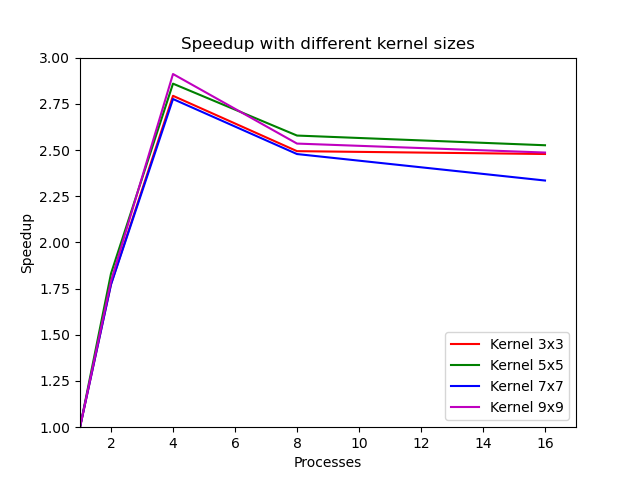
\includegraphics[width=\linewidth]{images/speedup_by_kernel_sizes.png}
	\caption{Speedup of the convolution function on a 734x694 image with different kernel sizes.}
	\label{fig:speedup_kernel}
\end{figure}

\begin{table}[H]
	\begin{center}
		\begin{tabular}{|c|c|c|}
			\hline
			Processes & Execution Time (s) & Speedup \\
			\hline
			1 & 6.774 & 1 \\
			2 & 3.818 & 1.774 \\
			4 & 2.425 & 2.793 \\
			8 & 2.716 & 2.494 \\
			16 & 2.733 & 2.478 \\
			\hline
		\end{tabular}
	\end{center}
	\caption{Execution Times for the 3x3 kernel.}
	\label{tab:speedup_k_1}
\end{table}

\begin{table}[H]
	\begin{center}
		\begin{tabular}{|c|c|c|}
			\hline
			Processes & Execution Time (s) & Speedup \\
			\hline
			1 & 15.947 & 1 \\
			2 & 8.707 & 1.831 \\
			4 & 5.578 & 2.859 \\
			8 & 6.185 & 2.578 \\
			16 & 6.314 & 2.526 \\
			\hline
		\end{tabular}
	\end{center}
	\caption{Execution Times for the 5x5 kernel.}
	\label{tab:speedup_k_2}
\end{table}

\begin{table}[H]
	\begin{center}
		\begin{tabular}{|c|c|c|}
			\hline
			Processes & Execution Time (s) & Speedup \\
			\hline
			1 & 29.415 & 1.000 \\
			2 & 16.599 & 1.772 \\
			4 & 10.597 & 2.776 \\
			8 & 11.870 & 2.478 \\
			16 & 12.599 & 2.335 \\
			\hline
		\end{tabular}
	\end{center}
	\caption{Execution Times for the 7x7 kernel.}
	\label{tab:speedup_k_3}
\end{table}

\begin{table}[H]
	\begin{center}
		\begin{tabular}{|c|c|c|}
			\hline
			Processes & Execution Time (s) & Speedup \\
			\hline
			1 & 47.220 & 1.000 \\
			2 & 26.368 & 1.791 \\
			4 & 16.220 & 2.911 \\
			8 & 18.629 & 2.535 \\
			16 & 18.993 & 2.486 \\
			\hline
		\end{tabular}
	\end{center}
	\caption{Execution Times for the 9x9 kernel.}
	\label{tab:speedup_k_4}
\end{table}

In Figure \ref{fig:speedup_kernel} we have the different speedups for different numbers of preocesses used and some common kernel sizes. We can see how the speedup increases up to 4 processes in a sub-linear way and slightly decrease for higher numbers of processes, but still stay above the value of 2.
 
The speedup values obtained are similar for all kernels, showing that this parallelization is independent from (small) kernel sizes.
For increasing kernel sizes.

\begin{figure}[H]
	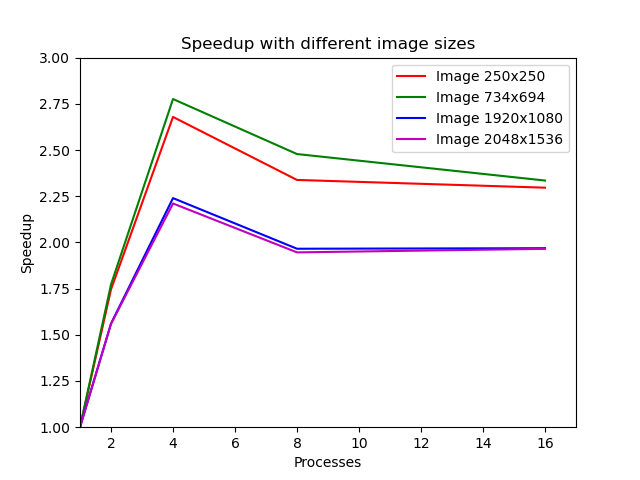
\includegraphics[width=\linewidth]{images/speedup_by_img_sizes.png}
	\caption{Speedup of the convolution function on a 7x7 kernel with different image sizes.}
	\label{fig:speedup_img}
\end{figure}

\begin{table}[H]
	\begin{center}
		\begin{tabular}{|c|c|c|}
			\hline
			Processes & Execution Time (s) & Speedup \\
			\hline
			1 & 3.429 & 1.000 \\
			2 & 1.965 & 1.745 \\
			4 & 1.280 & 2.679 \\
			8 & 1.467 & 2.338 \\
			16 & 1.494 & 2.296 \\
			\hline
		\end{tabular}
	\end{center}
	\caption{Execution Times for the 250x250 image.}
	\label{tab:speedup_k_i_1}
\end{table}

\begin{table}[H]
	\begin{center}
		\begin{tabular}{|c|c|c|}
			\hline
			Processes & Execution Time (s) & Speedup \\
			\hline
			1 & 29.415 & 1.000 \\
			2 & 16.599 & 1.772 \\
			4 & 10.597 & 2.776 \\
			8 & 11.870 & 2.478 \\
			16 & 12.599 & 2.335 \\
			\hline
		\end{tabular}
	\end{center}
	\caption{Execution Times for the 734x694 image.}
	\label{tab:speedup_k_i_2}
\end{table}

\begin{table}[H]
	\begin{center}
		\begin{tabular}{|c|c|c|}
			\hline
			Processes & Execution Time (s) & Speedup \\
			\hline
			1 & 124.920 & 1.000 \\
			2 & 80.047 & 1.561 \\
			4 & 55.777 & 2.240 \\
			8 & 63.549 & 1.966 \\
			16 & 63.456 & 1.969 \\
			\hline
		\end{tabular}
	\end{center}
	\caption{Execution Times for the 1920x1080 image.}
	\label{tab:speedup_i_3}
\end{table}

\begin{table}[H]
	\begin{center}
		\begin{tabular}{|c|c|c|}
			\hline
			Processes & Execution Time (s) & Speedup \\
			\hline
			1 & 189.372 & 1.000 \\
			2 & 121.490 & 1.559 \\
			4 & 85.668 & 2.211 \\
			8 & 97.315 & 1.946 \\
			16 & 96.365 & 1.965 \\
			\hline
		\end{tabular}
	\end{center}
	\caption{Execution Times for the 2048x1536 image.}
	\label{tab:speedup_i_4}
\end{table}

In Figure \ref{fig:speedup_img} we have the speedup trends for different input images. As before, the values increase up to 4 processes and decrease afterwards.

Bigger images tend to have less speedup overall, but still around 2 for more than 4 processes, making the parallel algorithm still more convenient than the sequential one.

\end{document}
